\documentclass[11pt]{article}

% =========================
% Packages
% =========================
\usepackage[margin=0.78in]{geometry}
\usepackage{amsmath,amssymb,amsfonts,mathtools}
\usepackage{booktabs,array,tabularx,longtable,multirow}
\usepackage{enumitem}
\usepackage[most]{tcolorbox}
\usepackage{xcolor}
\usepackage{fancyhdr}
\usepackage{titlesec}
\usepackage{hyperref}
\usepackage{lastpage}
\usepackage{setspace}
\usepackage{tikz}
\usepackage{pgfplots}
\usepackage{needspace}
\usepackage{caption}
\usepackage{multicol}
\usepackage{graphicx}
\usepackage{amsthm}
\usepackage{mathrsfs}
\usepackage{bm}
\usepackage{float}
\usepackage{colortbl}
\usepackage{tocloft}

\pgfplotsset{compat=1.18}
\setstretch{1.16}
\setlength{\parindent}{0pt}
\setlength{\parskip}{0.45em}
\setlist[itemize]{leftmargin=1.8em}
\setlist[enumerate]{leftmargin=2em}

% =========================
% Colors (Optimized Novel Prep Purple Theme)
% =========================
\definecolor{novelPurple}{RGB}{106,76,230}
\definecolor{novelPurpleDark}{RGB}{76,50,180}
\definecolor{novelPurpleLight}{RGB}{244,241,255}
\definecolor{novelPurpleLine}{RGB}{188,170,255}
\definecolor{npgray}{RGB}{78,78,78}
\definecolor{softgray}{RGB}{246,246,250}
\definecolor{softlav}{RGB}{250,248,255}
\definecolor{greencheck}{RGB}{24,128,88}
\definecolor{warmred}{RGB}{188,54,54}

% =========================
% Hyperref
% =========================
\hypersetup{
    colorlinks=true,
    linkcolor=novelPurpleDark,
    urlcolor=novelPurpleDark,
    citecolor=novelPurpleDark
}

% =========================
% Header / Footer
% =========================
\pagestyle{fancy}
\fancyhf{}
\fancyhead[L]{\textbf{Novel Prep Learning Center}}
\fancyhead[R]{\textbf{AP Calculus BC --- Unit 1}}
\fancyfoot[C]{\textcolor{novelPurpleDark}{\thepage\ /\ \pageref{LastPage}}}
\renewcommand{\headrulewidth}{0.4pt}
\renewcommand{\footrulewidth}{0pt}

% =========================
% TOC / Numbering Optimization
% =========================
\setcounter{secnumdepth}{2}
\setcounter{tocdepth}{2}
\renewcommand{\thesection}{1.\arabic{section}}
\renewcommand{\thesubsection}{1.\arabic{section}.\arabic{subsection}}
\renewcommand{\contentsname}{Contents}
\renewcommand{\cfttoctitlefont}{\Huge\bfseries\color{novelPurpleDark}}
\renewcommand{\cftaftertoctitle}{\hfill}
\renewcommand{\cftsecleader}{\cftdotfill{\cftdotsep}}
\renewcommand{\cftsubsecleader}{\cftdotfill{\cftdotsep}}
\setlength{\cftbeforesecskip}{7pt}
\setlength{\cftbeforesubsecskip}{2pt}
\setlength{\cftsecnumwidth}{3.2em}
\setlength{\cftsubsecnumwidth}{4.3em}
\renewcommand{\cftsecfont}{\color{novelPurpleDark}\bfseries}
\renewcommand{\cftsubsecfont}{\color{npgray}}
\renewcommand{\cftsecpagefont}{\color{novelPurpleDark}\bfseries}
\renewcommand{\cftsubsecpagefont}{\color{npgray}}

% =========================
% Section styles
% =========================
\titleformat{\section}
{\Large\bfseries\color{novelPurpleDark}}{\thesection.}{0.6em}{}

\titleformat{\subsection}
{\large\bfseries\color{novelPurple}}{\thesubsection.}{0.6em}{}

\titleformat{\subsubsection}
{\normalsize\bfseries\color{novelPurpleDark}}{}{0em}{}

% =========================
% tcolorbox styles
% =========================
\tcbset{
  enhanced,
  sharp corners,
  boxrule=0.95pt
}

% Main professional style: white body + purple title bar
\newtcolorbox{theorybox}[1]{
  colback=white,
  colframe=novelPurple,
  colbacktitle=novelPurple,
  coltitle=white,
  title={\large\textbf{#1}},
  fonttitle=\bfseries,
  sharp corners,
  enhanced,
  breakable,
  boxrule=0.95pt
}

% Soft note style
\newtcolorbox{notebox}[1]{
  colback=softlav,
  colframe=novelPurple,
  colbacktitle=novelPurple,
  coltitle=white,
  title={\large\textbf{#1}},
  fonttitle=\bfseries,
  sharp corners,
  enhanced,
  breakable,
  boxrule=0.95pt
}

% AP / skill / checkpoint style
\newtcolorbox{skillbox}[1]{
  colback=novelPurpleLight,
  colframe=novelPurpleDark,
  colbacktitle=novelPurpleDark,
  coltitle=white,
  title={\large\textbf{#1}},
  fonttitle=\bfseries,
  sharp corners,
  enhanced,
  breakable,
  boxrule=0.95pt
}

% Dedicated Big Idea box
\newtcolorbox{bigideabox}[1]{
  colback=white,
  colframe=novelPurple,
  colbacktitle=novelPurple,
  coltitle=white,
  title={\large\textbf{#1}},
  fonttitle=\bfseries,
  sharp corners,
  enhanced,
  breakable,
  boxrule=1pt
}

\newcommand{\ds}{\displaystyle}
\newcommand{\R}{\mathbb{R}}

% =========================
% Example formatting
% =========================
\newcounter{examplectr}[section]
\renewcommand{\theexamplectr}{\thesection.\arabic{examplectr}}

\newcommand{\example}[1]{%
\refstepcounter{examplectr}
\noindent{\color{novelPurpleDark}\textbf{Example \theexamplectr.}} \textbf{#1}
}

\newcommand{\solution}{\noindent{\textbf{Solution.}}}

\newcommand{\apcheckpoint}[1]{%
\begin{skillbox}{AP Checkpoint}
#1
\end{skillbox}
}

\begin{document}

% =========================================================
% COVER PAGE
% =========================================================
\begin{titlepage}
\centering
\vspace*{2.0cm}

{\fontsize{28}{32}\selectfont\bfseries\color{novelPurpleDark} AP Calculus AB\&BC\par}
\vspace{0.4cm}
{\fontsize{28}{32}\selectfont\bfseries\color{novelPurpleDark} Unit 1: Limits and Continuity\par}
\vspace{0.15cm}
{\Large\color{npgray} AP Calculus AB/BC Foundations\par}


\vspace{1.0cm}

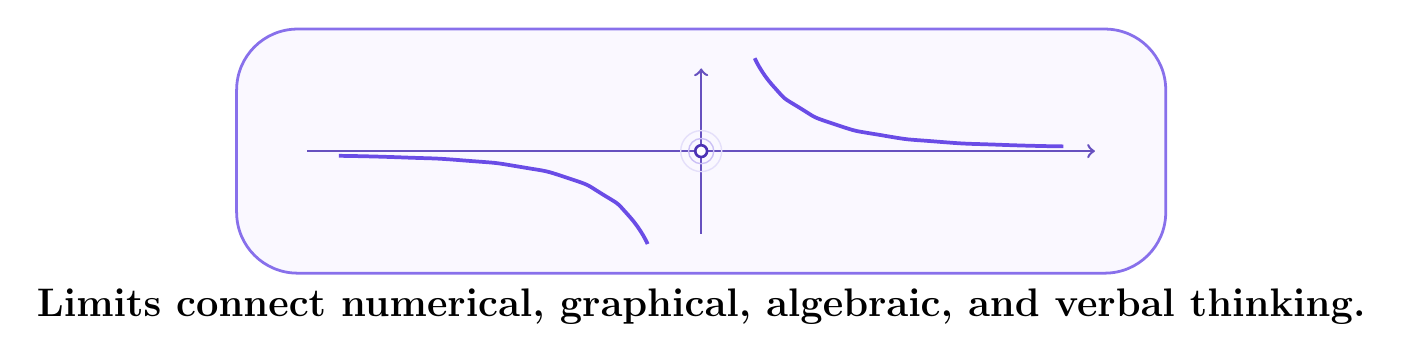
\begin{tikzpicture}[scale=1]

% background card
\fill[softlav, rounded corners=22pt] (-5.9,-1.55) rectangle (5.9,1.55);
\draw[novelPurple!80, line width=1pt, rounded corners=22pt] (-5.9,-1.55) rectangle (5.9,1.55);

% horizontal guide
\draw[novelPurpleDark!85, line width=0.9pt, ->] (-5.0,0) -- (5.0,0);

% vertical guide
\draw[novelPurpleDark!85, line width=0.9pt, ->] (0,-1.05) -- (0,1.05);

% left approaching curve
\draw[novelPurple, line width=1.35pt, smooth]
  plot [tension=1.05] coordinates {
    (-4.6,-0.06) (-3.8,-0.08) (-3.0,-0.12) (-2.3,-0.20)
    (-1.7,-0.34) (-1.25,-0.55) (-0.92,-0.82) (-0.68,-1.18)
  };

% right approaching curve
\draw[novelPurple, line width=1.35pt, smooth]
  plot [tension=1.05] coordinates {
    (0.68,1.18) (0.92,0.82) (1.25,0.55) (1.7,0.34)
    (2.3,0.20) (3.0,0.12) (3.8,0.08) (4.6,0.06)
  };

% center marker
\fill[white] (0,0) circle (0.075);
\draw[novelPurpleDark, line width=0.95pt] (0,0) circle (0.075);

% tiny glow rings for premium feel
\draw[novelPurple!35, line width=0.5pt] (0,0) circle (0.16);
\draw[novelPurple!18, line width=0.5pt] (0,0) circle (0.26);

% caption
\node[align=center, text=black] at (0,-1.98)
{\Large\bfseries Limits connect numerical, graphical, algebraic, and verbal thinking.};

\end{tikzpicture}
\vfill

\begin{minipage}{0.83\textwidth}
\begin{notebox}{Design Goals for This Revision}
\begin{itemize}
    \item Keep the overall spirit and progression of your original Unit 1.
    \item Upgrade the visual style to a cleaner Novel Prep purple theme.
    \item Expand the coverage so it aligns more fully with AP Calculus BC Unit 1.
    \item Improve explanation flow, examples, figures, and classroom usefulness.
    \item Build a more polished foundation for the rest of the textbook.
\end{itemize}
\end{notebox}
\end{minipage}

\vfill

{\large\textbf{Novel Prep Learning Center}}\\[0.25em]

\end{titlepage}

\clearpage
\thispagestyle{fancy}
\tableofcontents
\newpage

% =========================================================
% UNIT OVERVIEW
% =========================================================
\section*{Unit Overview}
\addcontentsline{toc}{section}{Unit Overview}

\begin{skillbox}{Unit 1 Structure}
This revised unit follows the broad development of your original textbook while expanding it to reflect the AP Calculus BC Unit 1 scope more completely. The chapter is organized around the following ideas:
\begin{enumerate}
    \item introducing change and instantaneous behavior
    \item defining limits and reading notation correctly
    \item estimating limits from graphs and tables
    \item evaluating limits with algebraic properties and algebraic manipulation
    \item selecting appropriate strategies, including the Squeeze Theorem
    \item connecting multiple representations of limits
    \item classifying discontinuities and studying continuity
    \item understanding infinite limits, vertical asymptotes, limits at infinity, and horizontal asymptotes
\end{enumerate}
\end{skillbox}

\begin{theorybox}{AP Unit 1 Topic Map}
\renewcommand{\arraystretch}{1.28}
\begin{tabularx}{\textwidth}{>{\bfseries}p{0.16\textwidth} X >{\raggedright\arraybackslash}p{0.28\textwidth}}
\toprule
Topic & Focus & Main Skill Emphasis \\
\midrule
1.1 & Introducing Calculus: Can Change Occur at an Instant? & interpret changing behavior conceptually \\
1.2 & Defining Limits and Using Limit Notation & read and communicate limit notation \\
1.3 & Estimating Limit Values from Graphs & graphical interpretation \\
1.4 & Estimating Limit Values from Tables & numerical interpretation \\
1.5 & Determining Limits Using Algebraic Properties & direct substitution and limit laws \\
1.6 & Determining Limits Using Algebraic Manipulation & factoring, rationalizing, common denominators \\
1.7 & Selecting Procedures for Determining Limits & choosing the best method \\
1.8 & Determining Limits Using the Squeeze Theorem & bounding arguments \\
1.9 & Connecting Multiple Representations of Limits & translation between forms \\
1.10 & Exploring Types of Discontinuities & classify non-continuity \\
1.11 & Defining Continuity at a Point & apply the 3-condition definition \\
1.12 & Confirming Continuity over an Interval & continuity on intervals and endpoints \\
1.13 & Removing Discontinuities & removable holes and redefining functions \\
1.14 & Infinite Limits and Vertical Asymptotes & behavior near excluded points \\
1.15 & Limits at Infinity and Horizontal Asymptotes & end behavior \\
\bottomrule
\end{tabularx}
\end{theorybox}

\begin{notebox}{Teaching Philosophy for This Unit}
Students should not learn limits as a list of tricks. They should see limits as the language that describes \emph{approach behavior}. In this unit, every major idea appears in multiple forms: graph, table, algebra, and words. That is the key to lasting understanding.
\end{notebox}

\newpage
\setcounter{section}{0}

% =========================================================
% 1.1
% =========================================================
\section{Introducing Calculus: Can Change Occur at an Instant?}

\begin{bigideabox}{Big Idea}
One of the central questions of calculus is this:

\begin{center}
\emph{How can we describe what is happening at an instant when change usually takes time?}
\end{center}

Average rate of change looks over an interval. Instantaneous change asks what happens at a single moment. Limits are the tool that make this possible.
\end{bigideabox}

Suppose a particle travels along a line and its position is
\[
s(t)=t^2+1.
\]
Over the interval from $t=2$ to $t=3$, the average rate of change is
\[
\frac{s(3)-s(2)}{3-2}=\frac{10-5}{1}=5.
\]
But what if we want the rate of change \emph{at} $t=2$ exactly? That leads to expressions such as
\[
\frac{s(2+h)-s(2)}{h}
\]
and then to the limit as $h\to 0$.

\example{Motivating instantaneous change with a secant slope.}

For
\[
s(t)=t^2+1,
\]
compute the average rate of change from $t=2$ to $t=2+h$, and simplify.

\bigskip

\solution

\[
\frac{s(2+h)-s(2)}{h}
=
\frac{(2+h)^2+1-(2^2+1)}{h}
\]
\[
=
\frac{4+4h+h^2+1-5}{h}
=
\frac{4h+h^2}{h}
=
4+h.
\]

So as $h\to 0$, the average rate of change approaches
\[
4.
\]

\bigskip

\apcheckpoint{Why is the expression $4+h$ more useful than the original fraction? Because after simplification, we can see what value the rate is approaching as the interval length shrinks.}

\newpage

% =========================================================
% 1.2
% =========================================================
\section{Defining Limits and Using Limit Notation}

\subsection{What a Limit Means}

\begin{theorybox}{Definition of a Limit (Informal)}
When we write
\[
\lim_{x\to c}f(x)=L,
\]
we mean that as $x$ gets arbitrarily close to $c$, the value of $f(x)$ gets arbitrarily close to $L$.
\end{theorybox}

\begin{theorybox}{Important Clarification}
A limit describes what the function is \emph{approaching}, not necessarily what the function \emph{equals} at the point.
\end{theorybox}

\begin{theorybox}{Formal Definition (Optional Precision)}
Let $f$ be defined on an open interval containing $c$, except possibly at $c$ itself. We say
\[
\lim_{x\to c}f(x)=L
\]
if for every $\varepsilon>0$, there exists a $\delta>0$ such that whenever
\[
0<|x-c|<\delta,
\]
it follows that
\[
|f(x)-L|<\varepsilon.
\]
\end{theorybox}

\subsection{Reading the Notation}

\[
\lim_{x\to 3}f(x)=5
\]
is read as:

\begin{center}
\emph{``The limit of $f(x)$ as $x$ approaches $3$ is $5$.''}
\end{center}

This does \emph{not} automatically mean that $f(3)=5$.

\example{Separating the function value from the limit value.}

Suppose
\[
f(x)=
\begin{cases}
x+2, & x\neq 3,\\[0.2em]
10, & x=3.
\end{cases}
\]
Find $\lim_{x\to 3}f(x)$ and compare it to $f(3)$.

\bigskip

\solution

For all $x\neq 3$, the function behaves like $x+2$. Therefore,
\[
\lim_{x\to 3}f(x)=\lim_{x\to 3}(x+2)=5.
\]
But by definition,
\[
f(3)=10.
\]

So
\[
\lim_{x\to 3}f(x)=5
\qquad\text{while}\qquad
f(3)=10.
\]

These are different.

\bigskip

\begin{notebox}{Key Message}
A function can have a limit at $x=c$ even if:
\begin{itemize}
    \item the function is not defined at $x=c$, or
    \item the function value at $x=c$ does not equal the limit.
\end{itemize}
\end{notebox}

\newpage

% =========================================================
% 1.3
% =========================================================
\section{Estimating Limit Values from Graphs}

\begin{theorybox}{Graphical Strategy}
To estimate
\[
\lim_{x\to c}f(x),
\]
look at the $y$-values the graph approaches from the left and from the right as $x$ gets close to $c$.
\end{theorybox}

\subsection{A Visual Example}

\begin{center}
\begin{tikzpicture}[scale=1.08]
\begin{axis}[
    axis lines=middle,
    xmin=-1.2,xmax=4.6,
    ymin=-0.8,ymax=4.8,
    width=12.2cm,
    height=7.0cm,
    xtick={0,1,2,3,4},
    ytick={0,1,2,3,4},
    xlabel={$x$},
    ylabel={$y$},
    every axis x label/.style={at={(current axis.right of origin)}, anchor=west},
    every axis y label/.style={at={(current axis.above origin)}, anchor=south},
    clip=false
]
\addplot[novelPurpleDark, very thick, domain=-1:2, samples=200] {x+1};
\addplot[novelPurpleDark, very thick, domain=2:4.4, samples=200] {-x+5};
\addplot[novelPurpleDark, only marks, mark=*, mark size=2.2pt] coordinates {(2,1.5)};
\addplot[novelPurpleDark, only marks, mark=o, mark size=2.4pt] coordinates {(2,3)};
\end{axis}
\end{tikzpicture}
\end{center}

From the graph:
\[
\lim_{x\to 2^-}f(x)=3,
\qquad
\lim_{x\to 2^+}f(x)=3.
\]
Therefore,
\[
\lim_{x\to 2}f(x)=3.
\]
But the solid point is at
\[
f(2)=1.5.
\]

\example{Reading a limit from a graph.}

Use the graph above to determine:
\[
\lim_{x\to 2}f(x),\qquad f(2),\qquad \text{and whether }f\text{ is continuous at }x=2.
\]

\bigskip

\solution

From both sides, the graph approaches $3$, so
\[
\lim_{x\to 2}f(x)=3.
\]
The solid point gives the actual function value:
\[
f(2)=1.5.
\]
Since
\[
\lim_{x\to 2}f(x)\neq f(2),
\]
the function is \textbf{not continuous} at $x=2$.

\bigskip

\begin{notebox}{Graph Checklist}
When reading from a graph, always ask:
\begin{enumerate}
    \item What does the graph approach from the left?
    \item What does the graph approach from the right?
    \item Are those two values equal?
    \item Is the actual point filled in somewhere else?
\end{enumerate}
\end{notebox}

\newpage

% =========================================================
% 1.4
% =========================================================
\section{Estimating Limit Values from Tables}

\begin{theorybox}{Numerical Strategy}
To estimate a limit numerically, evaluate the function at inputs close to the target value from both sides and look for the output values the function approaches.
\end{theorybox}

\example{Estimating a limit numerically.}

Estimate
\[
\lim_{x\to 0}\frac{x}{\sqrt{x+1}-1}.
\]

\bigskip

\solution

We first build a table of values near $x=0$.

\begin{center}
\renewcommand{\arraystretch}{1.2}
\begin{tabular}{c|ccccccc}
\toprule
$x$ & $-0.01$ & $-0.001$ & $-0.0001$ & $0$ & $0.0001$ & $0.001$ & $0.01$ \\
\midrule
$\ds \frac{x}{\sqrt{x+1}-1}$ & $1.99499$ & $1.99950$ & $1.99995$ & undefined & $2.00005$ & $2.00050$ & $2.00499$ \\
\bottomrule
\end{tabular}
\end{center}

The output values approach $2$ from both sides, so the limit appears to be
\[
\boxed{2}.
\]

\bigskip

\begin{notebox}{Important Warning}
A table provides evidence, not a proof. A numerical estimate can suggest a limit, but later in the unit we confirm limits algebraically when possible.
\end{notebox}

\example{A table where the limit does not exist.}

Suppose a table near $x=0$ for a function $g$ gives:

\begin{center}
\renewcommand{\arraystretch}{1.2}
\begin{tabular}{c|ccc|ccc}
\toprule
$x$ & $-0.1$ & $-0.01$ & $-0.001$ & $0.001$ & $0.01$ & $0.1$ \\
\midrule
$g(x)$ & $-1.01$ & $-1.00$ & $-1.00$ & $0.99$ & $1.00$ & $1.01$ \\
\bottomrule
\end{tabular}
\end{center}

What can you conclude about $\lim_{x\to 0}g(x)$?

\bigskip

\solution

From the left side, the values approach $-1$.
From the right side, the values approach $1$.

Since the left-hand and right-hand limits are different,
\[
\lim_{x\to 0}g(x)
\]
does not exist.

\newpage

% =========================================================
% 1.5
% =========================================================
\section{Determining Limits Using Algebraic Properties}

\begin{theorybox}{Some Basic Limits}
For real numbers $b,c$ and positive integer $n$:
\[
\lim_{x\to c} b=b,
\qquad
\lim_{x\to c} x=c,
\qquad
\lim_{x\to c} x^n=c^n.
\]
\end{theorybox}

\begin{theorybox}{Properties of Limits}
If
\[
\lim_{x\to c}f(x)=L
\qquad\text{and}\qquad
\lim_{x\to c}g(x)=K,
\]
then:
\begin{enumerate}
    \item $\lim\limits_{x\to c}[f(x)+g(x)]=L+K$
    \item $\lim\limits_{x\to c}[f(x)-g(x)]=L-K$
    \item $\lim\limits_{x\to c}[f(x)g(x)]=LK$
    \item $\lim\limits_{x\to c}\dfrac{f(x)}{g(x)}=\dfrac{L}{K}$ if $K\neq 0$
    \item $\lim\limits_{x\to c}[f(x)]^n=L^n$
\end{enumerate}
\end{theorybox}

\begin{theorybox}{Direct Substitution Principle}
If a function is continuous at $x=c$, then
\[
\lim_{x\to c}f(x)=f(c).
\]
This works for:
\begin{itemize}
    \item polynomials
    \item rational functions where the denominator is not zero
    \item radicals when the input stays in the domain
    \item many standard elementary functions
\end{itemize}
\end{theorybox}

\example{Evaluating basic limits by substitution.}

Find:
\[
\lim_{x\to 2}(4x^2+3).
\]

\bigskip

\solution

Since polynomials are continuous everywhere, substitute directly:
\[
\lim_{x\to 2}(4x^2+3)=4(2)^2+3=16+3=19.
\]

\[
\boxed{19}
\]

\bigskip

\example{A rational function with direct substitution.}

Find:
\[
\lim_{x\to 1}\frac{x^2+x+2}{x+1}.
\]

\bigskip

\solution

Because the denominator at $x=1$ is
\[
1+1=2\neq 0,
\]
the function is continuous at $x=1$. Substitute directly:
\[
\lim_{x\to 1}\frac{x^2+x+2}{x+1}
=
\frac{1^2+1+2}{1+1}
=
\frac{4}{2}=2.
\]

\[
\boxed{2}
\]

\bigskip

\example{A composite function.}

Find:
\[
\lim_{x\to 0}\sqrt{x^2+4}.
\]

\bigskip

\solution

First evaluate the inside:
\[
x^2+4\to 0^2+4=4.
\]
Then apply the outer function:
\[
\sqrt{x^2+4}\to \sqrt{4}=2.
\]

So
\[
\boxed{2}.
\]

\bigskip
\newpage
\begin{notebox}{Procedure Selection}
Before doing complicated algebra, first ask:
\begin{center}
\emph{Can I substitute directly?}
\end{center}
If yes, that is usually the fastest correct method.
\end{notebox}

\newpage

% =========================================================
% 1.6
% =========================================================
\section{Determining Limits Using Algebraic Manipulation}

Sometimes direct substitution leads to an indeterminate form such as
\[
\frac{0}{0}.
\]
In that case, the limit may still exist, but we need to rewrite the expression.

\begin{theorybox}{Most Common Algebraic Techniques}
\begin{enumerate}
    \item factoring and canceling common factors
    \item rationalizing with a conjugate
    \item combining fractions over a common denominator
    \item simplifying complex fractions
\end{enumerate}
\end{theorybox}

\subsection{Factoring}

\example{Factoring out a common factor.}

Find:
\[
\lim_{x\to 1}\frac{x^3-1}{x-1}.
\]

\bigskip

\solution

Direct substitution gives
\[
\frac{1^3-1}{1-1}=\frac00,
\]
so we factor:
\[
x^3-1=(x-1)(x^2+x+1).
\]
Thus
\[
\frac{x^3-1}{x-1}=x^2+x+1,\qquad x\neq 1.
\]
Now take the limit:
\[
\lim_{x\to 1}(x^2+x+1)=1+1+1=3.
\]

\[
\boxed{3}
\]

\subsection{Rationalizing}

\example{Rationalizing a radical expression.}

Find:
\[
\lim_{x\to 0}\frac{x}{\sqrt{x+1}-1}.
\]

\bigskip

\solution

Direct substitution gives
\[
\frac{0}{0},
\]
so multiply numerator and denominator by the conjugate:
\[
\frac{x}{\sqrt{x+1}-1}\cdot\frac{\sqrt{x+1}+1}{\sqrt{x+1}+1}
=
\frac{x(\sqrt{x+1}+1)}{(x+1)-1}.
\]
The denominator simplifies to $x$, so
\[
\frac{x(\sqrt{x+1}+1)}{x}=\sqrt{x+1}+1,\qquad x\neq 0.
\]
Now substitute:
\[
\lim_{x\to 0}(\sqrt{x+1}+1)=\sqrt{1}+1=2.
\]

\[
\boxed{2}
\]

\subsection{Combining Fractions}

\example{Common denominator method.}

Find:
\[
\lim_{x\to 0}\frac{\frac{1}{x+2}-\frac12}{x}.
\]

\bigskip

\solution

First combine the terms in the numerator:
\[
\frac{1}{x+2}-\frac12
=
\frac{2-(x+2)}{2(x+2)}
=
\frac{-x}{2(x+2)}.
\]
So
\[
\frac{\frac{1}{x+2}-\frac12}{x}
=
\frac{-x}{2(x+2)}\cdot \frac{1}{x}
=
-\frac{1}{2(x+2)}.
\]
Now substitute $x=0$:
\[
-\frac{1}{2(2)}=-\frac14.
\]

\[
\boxed{-\frac14}
\]

\bigskip

\apcheckpoint{If direct substitution gives $\frac00$, do not conclude the limit does not exist. Instead, look for algebraic simplification.}

\newpage

% =========================================================
% 1.7
% =========================================================
\section{Selecting Procedures for Determining Limits}

\begin{skillbox}{Strategy Ladder}
When evaluating a limit, use this decision order:
\begin{enumerate}
    \item \textbf{Try direct substitution.}
    \item If you get a real number, you are done.
    \item If you get $\frac00$, simplify algebraically.
    \item If the expression is bounded by two simpler expressions, consider the Squeeze Theorem.
    \item If the function is piecewise or graph-based, compare left- and right-hand behavior.
    \item If the variable goes to $\infty$ or $-\infty$, analyze end behavior.
\end{enumerate}
\end{skillbox}

\example{Choosing the right procedure.}

State the best method first, then evaluate:
\[
\lim_{x\to 4}\frac{x^2-16}{x-4}.
\]

\bigskip

\solution

Direct substitution gives
\[
\frac{16-16}{4-4}=\frac00,
\]
so the best method is \textbf{factoring}.

\[
x^2-16=(x-4)(x+4).
\]
Then
\[
\frac{x^2-16}{x-4}=x+4,\qquad x\neq 4.
\]
Now substitute:
\[
\lim_{x\to 4}(x+4)=8.
\]

\[
\boxed{8}
\]

\bigskip

\example{Choosing direct substitution instead.}

Evaluate:
\[
\lim_{x\to -2}(3x^3-5x+7).
\]

\bigskip

\solution

This is a polynomial, so direct substitution is the best method:
\[
3(-2)^3-5(-2)+7
=
3(-8)+10+7
=
-24+17=-7.
\]

\[
\boxed{-7}
\]

\newpage

% =========================================================
% 1.8
% =========================================================
\section{Determining Limits Using the Squeeze Theorem}

\begin{theorybox}{Squeeze Theorem}
If
\[
g(x)\le f(x)\le h(x)
\]
for all $x$ near $c$ (except possibly at $c$), and if
\[
\lim_{x\to c}g(x)=\lim_{x\to c}h(x)=L,
\]
then
\[
\lim_{x\to c}f(x)=L.
\]
\end{theorybox}

\begin{theorybox}{A Classic Bounding Fact}
Because
\[
-1\le \sin\theta \le 1
\]
for all real $\theta$, we often multiply by a quantity involving $x$ to create useful bounds.
\end{theorybox}

\example{A classic Squeeze Theorem problem.}

Find:
\[
\lim_{t\to 0} t^2\sin\!\left(\frac{1}{t}\right).
\]

\bigskip

\solution

Since
\[
-1\le \sin\left(\frac1t\right)\le 1,
\]
multiply everything by $t^2$.
Because $t^2\ge 0$ for all real $t$, the inequality direction stays the same:
\[
-t^2\le t^2\sin\left(\frac1t\right)\le t^2.
\]
Now take limits:
\[
\lim_{t\to 0}(-t^2)=0
\qquad\text{and}\qquad
\lim_{t\to 0}t^2=0.
\]
Therefore, by the Squeeze Theorem,
\[
\lim_{t\to 0} t^2\sin\left(\frac1t\right)=0.
\]

\[
\boxed{0}
\]

\bigskip
\newpage
\example{A trigonometric squeeze-based fact.}

A standard special limit is
\[
\lim_{x\to 0}\frac{\sin x}{x}=1.
\]
Use it to find:
\[
\lim_{x\to 0}\frac{\sin 4x}{x}.
\]

\bigskip

\solution

Rewrite the expression:
\[
\frac{\sin 4x}{x}
=
4\cdot \frac{\sin 4x}{4x}.
\]
As $x\to 0$, we also have $4x\to 0$, so
\[
\lim_{x\to 0}\frac{\sin 4x}{4x}=1.
\]
Therefore
\[
\lim_{x\to 0}\frac{\sin 4x}{x}
=
4(1)=4.
\]

\[
\boxed{4}
\]

\bigskip

\begin{theorybox}{Two Special Trigonometric Limits}
\[
\lim_{x\to 0}\frac{\sin x}{x}=1
\qquad\text{and}\qquad
\lim_{x\to 0}\frac{1-\cos x}{x}=0.
\]
\end{theorybox}

\newpage

% =========================================================
% 1.9
% =========================================================
\section{Connecting Multiple Representations of Limits}

\begin{theorybox}{Same Idea, Different Forms}
A limit can be represented:
\begin{itemize}
    \item graphically
    \item numerically (table)
    \item algebraically
    \item verbally
\end{itemize}
A strong AP student should be able to move smoothly between all four.
\end{theorybox}

\example{Connecting a graph, table, and formula.}

Suppose a function satisfies:
\[
f(x)=\frac{x^2-9}{x-3},\qquad x\neq 3.
\]
Describe the limit as $x\to 3$ in three ways.

\bigskip

\solution

\textbf{Algebraic view:}
\[
\frac{x^2-9}{x-3}=\frac{(x-3)(x+3)}{x-3}=x+3,\qquad x\neq 3.
\]
So
\[
\lim_{x\to 3}f(x)=6.
\]

\textbf{Numerical view:}
Values of $x$ near $3$ produce outputs near $6$.

\textbf{Graphical view:}
The graph follows the line $y=x+3$ with a hole at $(3,6)$, so the graph approaches $6$ as $x\to 3$.

\textbf{Verbal view:}
As the input approaches $3$, the output approaches $6$.

\bigskip

\apcheckpoint{A removable hole is one of the best examples for teaching that a limit depends on approach behavior, not just on whether the point itself is filled in.}

% =========================================================
% 1.10
% =========================================================
\section{Exploring Types of Discontinuities}

\begin{theorybox}{Three Common Types of Discontinuity}
\begin{enumerate}
    \item \textbf{Removable discontinuity:} the graph has a hole; the limit exists.
    \item \textbf{Jump discontinuity:} left- and right-hand limits are finite but unequal.
    \item \textbf{Infinite discontinuity:} the function grows without bound near a point.
\end{enumerate}
\end{theorybox}

\subsection{Visual Classification}

\begin{center}
\begin{tikzpicture}[scale=1]
% removable
\begin{scope}[shift={(-5.2,0)}]
\draw[->, thick] (-1.6,0) -- (1.6,0);
\draw[->, thick] (0,-1.3) -- (0,1.6);
\draw[novelPurpleDark, thick, domain=-1.4:1.4, samples=120] plot (\x,{0.55*\x+0.2});
\draw[novelPurpleDark, fill=white, thick] (0.5,0.475) circle (0.07);
\node at (0,-1.8) {\small Removable};
\end{scope}

% jump
\begin{scope}[shift={(0,0)}]
\draw[->, thick] (-1.6,0) -- (1.6,0);
\draw[->, thick] (0,-1.3) -- (0,1.6);
\draw[novelPurpleDark, thick] (-1.3,-0.6) -- (0,-0.6);
\draw[novelPurpleDark, thick] (0,0.7) -- (1.3,0.7);
\draw[novelPurpleDark, fill=white, thick] (0,-0.6) circle (0.07);
\draw[novelPurpleDark, fill=white, thick] (0,0.7) circle (0.07);
\node at (0,-1.8) {\small Jump};
\end{scope}

% infinite
\begin{scope}[shift={(5.2,0)}]
\draw[->, thick] (-1.6,0) -- (1.6,0);
\draw[->, thick] (0,-1.3) -- (0,1.6);
\draw[dashed, novelPurpleLine, thick] (0,-1.2) -- (0,1.5);
\draw[novelPurpleDark, thick, domain=-1.35:-0.14, samples=120] plot (\x,{0.2/(\x)});
\draw[novelPurpleDark, thick, domain=0.14:1.35, samples=120] plot (\x,{0.2/(\x)});
\node at (0,-1.8) {\small Infinite};
\end{scope}
\end{tikzpicture}
\end{center}

\example{Classifying discontinuities.}

Classify the discontinuity at the indicated point.

\begin{enumerate}
    \item $\ds f(x)=\frac{x^2-4}{x-2}$ at $x=2$
    \item $\ds g(x)=\frac{|x|}{x}$ at $x=0$
    \item $\ds h(x)=\frac{1}{x^2}$ at $x=0$
\end{enumerate}

\bigskip

\solution

\textbf{1.}
\[
\frac{x^2-4}{x-2}=\frac{(x-2)(x+2)}{x-2}=x+2,\qquad x\neq 2.
\]
The graph has a hole at $x=2$, so this is a \textbf{removable discontinuity}.

\textbf{2.} The left-hand limit is $-1$ and the right-hand limit is $1$, so the function has a \textbf{jump discontinuity}.

\textbf{3.} As $x\to 0$, the function grows without bound, so this is an \textbf{infinite discontinuity}.

\newpage

% =========================================================
% 1.11
% =========================================================
\section{Defining Continuity at a Point}

\begin{theorybox}{Continuity at a Point}
A function $f$ is continuous at $x=c$ if all three conditions are true:
\begin{enumerate}
    \item $f(c)$ is defined.
    \item $\lim\limits_{x\to c}f(x)$ exists.
    \item $\lim\limits_{x\to c}f(x)=f(c)$.
\end{enumerate}
\end{theorybox}

\example{Testing continuity with the three-condition definition.}

Determine whether
\[
f(x)=
\begin{cases}
\dfrac{x^2-x-2}{x-2}, & x\neq 2,\\[0.6em]
1, & x=2
\end{cases}
\]
is continuous at $x=2$.

\bigskip

\solution

\textbf{Condition 1:} $f(2)$ is defined, and
\[
f(2)=1.
\]

\textbf{Condition 2:} For $x\neq 2$,
\[
\frac{x^2-x-2}{x-2}
=
\frac{(x-2)(x+1)}{x-2}=x+1.
\]
So
\[
\lim_{x\to 2}f(x)=\lim_{x\to 2}(x+1)=3.
\]

\textbf{Condition 3:} Compare:
\[
\lim_{x\to 2}f(x)=3
\qquad\text{but}\qquad
f(2)=1.
\]
Since these are not equal, the function is \textbf{not continuous} at $x=2$.

\bigskip

\begin{notebox}{Fast Continuity Test}
Whenever a function is built from standard continuous functions and no domain restriction is violated, it is continuous automatically. But for piecewise functions and rational functions at excluded values, use the 3-condition definition carefully.
\end{notebox}

% =========================================================
% 1.12
% =========================================================
\newpage
\section{Confirming Continuity over an Interval}

\subsection{Open Intervals}

A function is continuous on an open interval $(a,b)$ if it is continuous at every point in that interval.

\subsection{Closed Intervals}

\begin{theorybox}{Continuity on a Closed Interval}
A function is continuous on $[a,b]$ if:
\begin{enumerate}
    \item it is continuous on $(a,b)$,
    \item $\lim\limits_{x\to a^+}f(x)=f(a)$,
    \item $\lim\limits_{x\to b^-}f(x)=f(b)$.
\end{enumerate}
\end{theorybox}

\begin{theorybox}{One-Sided Limits}
\[
\lim_{x\to c^-}f(x)=L
\quad\text{means the left-hand limit}
\]
and
\[
\lim_{x\to c^+}f(x)=L
\quad\text{means the right-hand limit.}
\]
A two-sided limit exists exactly when the left-hand and right-hand limits both exist and are equal.
\end{theorybox}

\example{Continuity on a closed interval.}

Discuss the continuity of
\[
f(x)=\sqrt{1-x^2}.
\]

\bigskip

\solution

The domain is
\[
-1\le x\le 1,
\]
so the function is defined on the closed interval $[-1,1]$.

Inside the interval, the square-root function composed with $1-x^2$ is continuous wherever defined, so $f$ is continuous on $(-1,1)$.

Now check the endpoints:
\[
\lim_{x\to -1^+}\sqrt{1-x^2}=0=f(-1),
\]
and
\[
\lim_{x\to 1^-}\sqrt{1-x^2}=0=f(1).
\]

Therefore, $f$ is continuous on
\[
\boxed{[-1,1]}.
\]

\newpage

% =========================================================
% 1.13
% =========================================================
\section{Removing Discontinuities}

\begin{theorybox}{Removable Discontinuity Idea}
If a limit exists at $x=c$ but the function is either undefined there or defined incorrectly there, then the discontinuity can be removed by redefining the function value to equal the limit.
\end{theorybox}

\example{Making a function continuous by redefining one point.}

Find a value of $k$ that makes
\[
f(x)=
\begin{cases}
\dfrac{x^2-9}{x-3}, & x\neq 3,\\[0.6em]
k, & x=3
\end{cases}
\]
continuous at $x=3$.

\bigskip

\solution

To be continuous at $x=3$, we need
\[
k=\lim_{x\to 3}\frac{x^2-9}{x-3}.
\]
Factor:
\[
\frac{x^2-9}{x-3}
=
\frac{(x-3)(x+3)}{x-3}=x+3,\qquad x\neq 3.
\]
So
\[
\lim_{x\to 3}\frac{x^2-9}{x-3}
=
\lim_{x\to 3}(x+3)=6.
\]
Thus the required value is
\[
\boxed{k=6}.
\]

\bigskip

\apcheckpoint{This is one of the most important continuity templates in AP Calculus: simplify first, find the limit, then define the missing point to match it.}

% =========================================================
% 1.14
% =========================================================
\newpage
\section{Infinite Limits and Vertical Asymptotes}

\begin{theorybox}{Infinite Limits}
If the values of $f(x)$ increase without bound as $x$ approaches $c$, we write
\[
\lim_{x\to c}f(x)=\infty.
\]
If the values decrease without bound, we write
\[
\lim_{x\to c}f(x)=-\infty.
\]
\end{theorybox}

\begin{theorybox}{Vertical Asymptotes}
If at least one of
\[
\lim_{x\to c^-}f(x),\qquad \lim_{x\to c^+}f(x)
\]
is $\infty$ or $-\infty$, then the line
\[
x=c
\]
is a vertical asymptote.
\end{theorybox}

\example{Finding a vertical asymptote.}

Determine the behavior of
\[
f(x)=\frac{1}{x-2}
\]
as $x\to 2^-$ and as $x\to 2^+$.

\bigskip

\solution

As $x\to 2^-$, the denominator $x-2$ is a very small negative number, so
\[
\frac{1}{x-2}\to -\infty.
\]

As $x\to 2^+$, the denominator $x-2$ is a very small positive number, so
\[
\frac{1}{x-2}\to \infty.
\]

Therefore,
\[
\lim_{x\to 2^-}\frac{1}{x-2}=-\infty,
\qquad
\lim_{x\to 2^+}\frac{1}{x-2}=\infty,
\]
and the graph has a vertical asymptote at
\[
\boxed{x=2}.
\]

\bigskip

\example{A rational function with a common factor.}

Determine all vertical asymptotes of
\[
f(x)=\frac{x^2+2x-8}{x^2-4}.
\]

\bigskip

\solution

Factor numerator and denominator:
\[
x^2+2x-8=(x+4)(x-2),
\qquad
x^2-4=(x+2)(x-2).
\]
So
\[
f(x)=\frac{(x+4)(x-2)}{(x+2)(x-2)}=\frac{x+4}{x+2},\qquad x\neq 2.
\]

The factor $x-2$ cancels, so $x=2$ is a hole, not a vertical asymptote.

The denominator of the simplified form is zero at $x=-2$, so
\[
x=-2
\]
is the vertical asymptote.

Thus the only vertical asymptote is
\[
\boxed{x=-2}.
\]

\newpage

% =========================================================
% 1.15
% =========================================================
\section{Limits at Infinity and Horizontal Asymptotes}

\begin{theorybox}{Limits at Infinity}
Limits at infinity describe how a function behaves as
\[
x\to \infty
\qquad\text{or}\qquad
x\to -\infty.
\]
These are end-behavior questions.
\end{theorybox}

\begin{theorybox}{Horizontal Asymptotes}
If
\[
\lim_{x\to\infty}f(x)=L
\quad\text{or}\quad
\lim_{x\to-\infty}f(x)=L,
\]
then the line
\[
y=L
\]
is a horizontal asymptote.
\end{theorybox}

\subsection{Rational Functions and End Behavior}

For rational functions, compare degrees:

\begin{itemize}
    \item If degree of numerator $<$ degree of denominator, then
    \[
    \lim_{x\to\pm\infty}f(x)=0.
    \]
    \item If degrees are equal, the limit is the ratio of leading coefficients.
    \item If degree of numerator $>$ degree of denominator, there is no horizontal asymptote.
\end{itemize}

\example{A zero horizontal asymptote.}

Find
\[
\lim_{x\to\infty}\frac{3x+1}{x^2+4}.
\]

\bigskip

\solution

The numerator has degree $1$, while the denominator has degree $2$. Since the denominator grows faster,
\[
\lim_{x\to\infty}\frac{3x+1}{x^2+4}=0.
\]
So the horizontal asymptote is
\[
\boxed{y=0}.
\]

\bigskip

\example{A ratio of leading coefficients.}

Find
\[
\lim_{x\to\infty}\frac{4x^2-7}{2x^2+5x+1}.
\]

\bigskip

\solution

The degrees are equal, so the limit is the ratio of leading coefficients:
\[
\lim_{x\to\infty}\frac{4x^2-7}{2x^2+5x+1}
=
\frac{4}{2}=2.
\]
Thus the horizontal asymptote is
\[
\boxed{y=2}.
\]

\bigskip

\example{Connecting horizontal asymptotes with graphs.}

Sketch the end behavior of a function satisfying
\[
\lim_{x\to\infty}f(x)=1
\qquad\text{and}\qquad
\lim_{x\to-\infty}f(x)=1.
\]

\bigskip

\solution

Both ends of the graph approach the line
\[
y=1.
\]
So $y=1$ is the horizontal asymptote.

\begin{center}
\begin{tikzpicture}
\begin{axis}[
    axis lines=middle,
    xmin=-5.3,xmax=5.3,
    ymin=-1.0,ymax=3.0,
    width=11.8cm,
    height=6.6cm,
    xtick={-4,-2,0,2,4},
    ytick={0,1,2},
    xlabel={$x$},
    ylabel={$y$},
    every axis x label/.style={at={(current axis.right of origin)}, anchor=west},
    every axis y label/.style={at={(current axis.above origin)}, anchor=south},
]
\addplot[dashed, novelPurpleLine, thick, domain=-5.2:5.2] {1};
\addplot[novelPurpleDark, very thick, domain=-5:5, samples=200] {1 + 1/(x^2+1)};
\end{axis}
\end{tikzpicture}
\end{center}

\newpage

% =========================================================
% SYNTHESIS
% =========================================================
\section*{Unit 1 Synthesis}
\addcontentsline{toc}{section}{Unit 1 Synthesis}

\begin{theorybox}{Unit 1 Summary of Core Definitions}
\textbf{Limit:}
\[
\lim_{x\to c}f(x)=L
\]
means $f(x)$ approaches $L$ as $x$ approaches $c$.

\textbf{Continuity at a point:}
\begin{enumerate}
    \item $f(c)$ exists
    \item $\lim\limits_{x\to c}f(x)$ exists
    \item $\lim\limits_{x\to c}f(x)=f(c)$
\end{enumerate}

\textbf{Vertical asymptote:}
\[
x=c
\]
when the function grows without bound near $x=c$.

\textbf{Horizontal asymptote:}
\[
y=L
\]
when $f(x)\to L$ as $x\to \pm\infty$.
\end{theorybox}

\begin{skillbox}{What Students Should Be Able To Do by the End of Unit 1}
\begin{itemize}
    \item interpret limits verbally, graphically, numerically, and algebraically
    \item distinguish between a limit value and a function value
    \item estimate limits from graphs and tables
    \item evaluate limits by direct substitution when allowed
    \item use factoring, conjugates, and common denominators for indeterminate forms
    \item choose the most efficient procedure for a given limit
    \item apply the Squeeze Theorem in classic AP situations
    \item classify removable, jump, and infinite discontinuities
    \item test continuity at a point and over an interval
    \item identify vertical and horizontal asymptotes
\end{itemize}
\end{skillbox}

\begin{notebox}{Most Important Unit 1 Habits}
\begin{enumerate}
    \item Do not confuse \emph{approaches} with \emph{equals}.
    \item Always test direct substitution first.
    \item If you get $\frac00$, simplify algebraically.
    \item For a two-sided limit, compare the left and right sides.
    \item A hole does not prevent the limit from existing.
    \item A vertical asymptote comes from unbounded behavior, not just from making a denominator zero before simplification.
\end{enumerate}
\end{notebox}

% =========================================================
% PRACTICE
% =========================================================
\newpage
\section*{Guided Practice Set}
\addcontentsline{toc}{section}{Guided Practice Set}

\example{Estimate graphically.}

Suppose a graph approaches $4$ from both sides as $x\to -1$, but the filled point is at $(-1,7)$. State:
\[
\lim_{x\to -1}f(x)
\qquad\text{and}\qquad
f(-1).
\]

\bigskip

\solution

\[
\lim_{x\to -1}f(x)=4
\qquad\text{and}\qquad
f(-1)=7.
\]

\bigskip

\example{Direct substitution.}

Find:
\[
\lim_{x\to 3}(2x^2-5x+1).
\]

\bigskip

\solution

\[
2(3)^2-5(3)+1=18-15+1=4.
\]

\[
\boxed{4}
\]

\bigskip

\example{Factoring.}

Find:
\[
\lim_{x\to 5}\frac{x^2-25}{x-5}.
\]

\bigskip

\solution

\[
x^2-25=(x-5)(x+5).
\]
So
\[
\frac{x^2-25}{x-5}=x+5,\qquad x\neq 5.
\]
Therefore,
\[
\lim_{x\to 5}(x+5)=10.
\]

\[
\boxed{10}
\]

\bigskip

\example{One-sided limits.}

Find
\[
\lim_{x\to 0^-}\frac{|x|}{x}
\qquad\text{and}\qquad
\lim_{x\to 0^+}\frac{|x|}{x}.
\]

\bigskip

\solution

If $x<0$, then $|x|=-x$, so
\[
\frac{|x|}{x}=\frac{-x}{x}=-1.
\]
Thus
\[
\lim_{x\to 0^-}\frac{|x|}{x}=-1.
\]

If $x>0$, then $|x|=x$, so
\[
\frac{|x|}{x}=1.
\]
Thus
\[
\lim_{x\to 0^+}\frac{|x|}{x}=1.
\]

\bigskip

\example{Continuity.}

Is
\[
f(x)=\frac{x+1}{x^2+4}
\]
continuous at $x=2$?

\bigskip

\solution

This is a rational function with denominator
\[
2^2+4=8\neq 0,
\]
so it is continuous at $x=2$.

\[
\boxed{\text{Yes}}
\]

\newpage

% =========================================================
% EXERCISES
% =========================================================
\section*{Homework / Class Exercises}
\addcontentsline{toc}{section}{Homework / Class Exercises}

\subsection*{Part A --- Core Practice}

\begin{enumerate}
    \item State in words what
    \[
    \lim_{x\to 4}f(x)=7
    \]
    means.

    \item Use direct substitution to evaluate:
    \[
    \lim_{x\to -2}(x^3+4x^2-1).
    \]

    \item Estimate from the expression by simplification:
    \[
    \lim_{x\to 2}\frac{x^2-4}{x-2}.
    \]

    \item Evaluate:
    \[
    \lim_{x\to 0}\frac{\sqrt{x+4}-2}{x}.
    \]

    \item Show that
    \[
    \lim_{x\to 0}\frac{|x|}{x}
    \]
    does not exist.

    \item Find a value of $k$ that makes the function continuous at $x=1$:
    \[
    f(x)=
    \begin{cases}
    \dfrac{x^2-1}{x-1}, & x\neq 1,\\[0.6em]
    k, & x=1.
    \end{cases}
    \]

    \item Determine whether the discontinuity of
    \[
    f(x)=\frac{x^2-1}{x-1}
    \]
    at $x=1$ is removable, jump, or infinite.

    \item Determine the vertical asymptote(s) of
    \[
    g(x)=\frac{x+3}{x^2-x-6}.
    \]

    \item Find the horizontal asymptote of
    \[
    h(x)=\frac{5x^2-3x+2}{2x^2+1}.
    \]

    \item Evaluate:
    \[
    \lim_{x\to 0}\frac{\sin 7x}{x}.
    \]
\end{enumerate}

\subsection*{Part B --- AP Style Mixed Reasoning}

\begin{enumerate}[start=11]
    \item A function $f$ satisfies:
    \[
    \lim_{x\to 3^-}f(x)=5,
    \qquad
    \lim_{x\to 3^+}f(x)=5,
    \qquad
    f(3)=-2.
    \]
    Does $\lim\limits_{x\to 3}f(x)$ exist? Is $f$ continuous at $x=3$?

    \item Find:
    \[
    \lim_{x\to \infty}\frac{3x^3+1}{x^2-4}.
    \]
    Explain whether there is a horizontal asymptote.

    \item Use the Squeeze Theorem to evaluate:
    \[
    \lim_{x\to 0}x\cos\left(\frac{1}{x}\right).
    \]

    \item For
    \[
    f(x)=
    \begin{cases}
    x+2, & x<1,\\
    4, & x=1,\\
    3x-1, & x>1,
    \end{cases}
    \]
    determine whether $f$ is continuous at $x=1$.

    \item Explain the difference between:
    \[
    \lim_{x\to c}f(x)
    \qquad\text{and}\qquad
    f(c).
    \]
\end{enumerate}

\newpage

% =========================================================
% ANSWER KEY
% =========================================================
\section*{Answer Key / Instructor Notes}
\addcontentsline{toc}{section}{Answer Key / Instructor Notes}

\textbf{1.} It means the outputs of $f(x)$ get arbitrarily close to $7$ as $x$ gets arbitrarily close to $4$.

\bigskip

\textbf{2.}
\[
(-2)^3+4(-2)^2-1=-8+16-1=7.
\]
\[
\boxed{7}
\]

\bigskip

\textbf{3.}
\[
\frac{x^2-4}{x-2}=\frac{(x-2)(x+2)}{x-2}=x+2.
\]
So the limit is
\[
4.
\]

\[
\boxed{4}
\]

\bigskip

\textbf{4.}
Rationalize:
\[
\frac{\sqrt{x+4}-2}{x}\cdot \frac{\sqrt{x+4}+2}{\sqrt{x+4}+2}
=
\frac{x+4-4}{x(\sqrt{x+4}+2)}
=
\frac{1}{\sqrt{x+4}+2}.
\]
Now let $x\to 0$:
\[
\frac{1}{2+2}=\frac14.
\]

\[
\boxed{\frac14}
\]

\bigskip

\textbf{5.}
\[
\lim_{x\to 0^-}\frac{|x|}{x}=-1,
\qquad
\lim_{x\to 0^+}\frac{|x|}{x}=1.
\]
Since they are different, the two-sided limit does not exist.

\bigskip

\textbf{6.}
\[
\frac{x^2-1}{x-1}=\frac{(x-1)(x+1)}{x-1}=x+1.
\]
So
\[
k=\lim_{x\to 1}(x+1)=2.
\]

\[
\boxed{k=2}
\]

\bigskip

\textbf{7.}
The factor cancels and leaves a hole, so the discontinuity is \textbf{removable}.

\bigskip

\textbf{8.}
\[
x^2-x-6=(x-3)(x+2).
\]
Thus the vertical asymptotes occur at
\[
x=3,\qquad x=-2.
\]

\[
\boxed{x=3,\,-2}
\]

\bigskip

\textbf{9.}
Degrees are equal, so the horizontal asymptote is the ratio of leading coefficients:
\[
y=\frac52.
\]

\[
\boxed{y=\frac52}
\]

\bigskip

\textbf{10.}
\[
\frac{\sin 7x}{x}
=
7\cdot\frac{\sin 7x}{7x}\to 7.
\]

\[
\boxed{7}
\]

\bigskip

\textbf{11.}
Yes,
\[
\lim_{x\to 3}f(x)=5
\]
exists because the two one-sided limits agree. But $f(3)=-2$, so the function is \textbf{not continuous} at $x=3$.

\bigskip

\textbf{12.}
The degree of the numerator is greater than the degree of the denominator, so the function grows without bound in magnitude. There is \textbf{no horizontal asymptote}. The limit is not finite.

\bigskip

\textbf{13.}
Since
\[
-1\le \cos\left(\frac1x\right)\le 1,
\]
multiplying by $x$ and squeezing carefully leads to
\[
-x\le x\cos\left(\frac1x\right)\le x
\quad\text{if }x>0,
\]
and similarly the bound still forces the expression to $0$ from both sides. Thus:
\[
\boxed{0}
\]

\bigskip

\textbf{14.}
Left-hand limit:
\[
\lim_{x\to 1^-}f(x)=1+2=3.
\]
Right-hand limit:
\[
\lim_{x\to 1^+}f(x)=3(1)-1=2.
\]
Since these are not equal, the limit does not exist, so the function is \textbf{not continuous} at $x=1$.

\bigskip

\textbf{15.}
$\lim_{x\to c}f(x)$ describes the value the function approaches near $x=c$, while $f(c)$ is the actual defined output at $x=c$. They may be equal, but they do not have to be.

% =========================================================
% FINAL PAGE
% =========================================================
\newpage
\section*{Unit 1 Final Teaching Checklist}
\addcontentsline{toc}{section}{Unit 1 Final Teaching Checklist}

\begin{skillbox}{Before Moving to Derivatives, Students Should Comfortably Handle}
\begin{itemize}
    \item interpreting limits from graphs and tables
    \item distinguishing the function value from the limiting value
    \item evaluating limits by direct substitution and by algebraic manipulation
    \item using one-sided limits
    \item classifying discontinuities
    \item checking continuity at points and on intervals
    \item recognizing vertical and horizontal asymptotes
\end{itemize}
\end{skillbox}

\vfill

\begin{center}
{\Large\bfseries\color{novelPurpleDark} End of Unit 1}\\[0.5em]
{\large\color{novelPurple} Limits and Continuity}
\end{center}

\end{document}


